% TODO:

% Write ``Liquid-vapor interface'' section A.

% Look up question-mark references (citations).

\documentclass[letterpaper,twocolumn,amsmath,amssymb,jcp,10pt,aip]{revtex4-1}
\usepackage{graphicx}% Include figure files
\usepackage{dcolumn}% Align table columns on decimal point
\usepackage{bm}% bold math
\usepackage{color}

\newcommand{\red}[1]{{\bf \color{red} #1}}
\newcommand{\blue}[1]{{\bf \color{blue} #1}}
\newcommand{\green}[1]{{\bf \color{green} #1}}
\newcommand{\rr}{\textbf{r}}
\newcommand{\refnote}{\red{[ref]}}

\newcommand{\fixme}[1]{\red{[#1]}}

%\newcommand{\derivation}[1]{#1} % Use this to show all derivations in detail
\newcommand{\derivation}[1]{} % Use this for nice pegagogical paper...

% needsworklater is used to annotate bits that need work, but that we
% can postpone for a while.
\newcommand{\needsworklater}[1]{\emph{[#1]}}
% needsworknow is intended to prioritize stuff that needs fixing.
\newcommand{\needsworknow}[1]{\textcolor{red}{[\emph{#1}]}}

\begin{document}
\title{A Fundamental Measure Theory Functional for Hard-Sphere Contact Densities}

\author{Jeff Schulte}
\author{Chris Haglund}
\author{Patrick Kreitzburg}
\author{David Roundy}
\affiliation{Department of Physics, Oregon State University, Corvallis, OR 97331}


%%%%%%%%%%%%%%%%%%%%%%%%%%%%%%%%%%%%%%%%%%%%%%%%%%%%%%%%%%%%
\begin{abstract}
  We investigate the contact density of an inhomogeneous hard-sphere
  fluid, which is of particular interest, as it plays a critical role
  in Statistical Associating Fluid Theory (SAFT), which is the basis
  of a number of recent classical density functionals.  We derive a
  formula for the contact density from the White Bear version of the
  Fundamental Measure Theory functional~\cite{roth2002whitebear}, and
  test this functional agains Monte Carlo simulations.
  \textcolor{red}{Insert summary of results here...}
\end{abstract}

\maketitle

%%%%%%%%%%%%%%%%%%%%%%%%%%%%%%%%%%%%%%%%%%%%%%%%%%%%%%%%%%%%
\section{Introduction}

\fixme{Figure out whether to stick with both $R$ and $\sigma$, or move
to only $\sigma$ in the paper, which would have a certain appeal.}

% The following are papers that use a SAFT-based classical DFT with at
% least some of the terms purely local
\newcommand\saftlocaldft{felipe2001examination, gloor2002saft,%
  gloor2004accurate, clark2006developing, gloor2007prediction,%
  kahl2008modified, gross2009density}
% The following are papers that use a SAFT-based classical DFT with
% all the terms that should be non-local being non-local.
\newcommand\saftnonlocaldft{yu2002fmt-dft-inhomogeneous-associating,%
  fu2005vapor-liquid-dft,bryk2006density}

There has been considerable recent interest in using Statistical
Associating Fluid Theory (SAFT) to construct classical density
functionals to describe associating
fluids\cite{\saftlocaldft,\saftnonlocaldft}.  This approach has been
successful in qualitatively describing the dependence of surface
tension on temperature.  Unfortunately, most of these constructed
functionals\cite{\saftlocaldft} cannot be used to study arbitrary
inhomogeneous density distributions, because they use local density
approximations that are only valid for densities that vary slowly over
molecular length scales.  A key input to those SAFT-based functionals
that can handle sharply varying densities is the correlation function
evaluated at contact.

Constructing a classical density functional based on SAFT involves
rewriting each term in the free energy as a functional of an
inhomogeneous density.  The SAFT free energy consists of four terms:
\begin{align}
  A_\textit{SAFT} &= A_\textit{ideal} + A_\textit{HS} + A_\textit{chain} + A_\textit{disp} + A_\textit{assoc}
\end{align}
where $A_\textit{ideal}$ is the ideal-gas free energy, $A_\textit{HS}$
is the excess free energy of a hard-sphere fluid of monomers,
$A_\textit{chain}$ is the contribution to the free energy from the
chaining effect in a polymeric fluid, $A_\textit{disp}$ is the
dispersion contribution to the free energy, and $A_\textit{assoc}$ is
the free energy contribution from \emph{association}, which is to say,
hydrogen bonding.  The chain and association contributions to the SAFT
free energy are of particular interest for this paper, since each uses
as input the contact value of the correlation function.
%
Yu and Wu introduced in 2002 a functional for the association term of
the free energy, which included a functional for the contact value of
the correlation function (see
Section~\ref{sec:yuwu})\cite{yu2002fmt-dft-inhomogeneous-associating},
which has subsequently been used in other
functionals\cite{fu2005vapor-liquid-dft, bryk2006density}.
%% Each of these terms has some dependence on the
%% inhomogeneity in the density.  The ideal gas is purely local, and in
%% fact must be the only purely local term in the free energy in order
%% for the functional to satisfy the contact-value theorem.  The
%% hard-sphere contribution contribution to the free energy has been
%% thoroughly studied, and is well approximated by the White Bear version
%% of the Fundamental-Measure Theory (FMT)
%% functional\cite{roth2002whitebear}.
Two functionals for the chain contribution have recently been
introduced\cite{bryk2006density, gross2009density}, one which uses the
contact value of the correlation function of Yu and
Wu\cite{bryk2006density}, while the other introduces a new functional
for the contact value of the correlation
function (see Section~\ref{sec:gross})\cite{gross2009density}.
%% The dispersion term is long-range and thus has significant
%% dependence on the density distribution, but because its relatively
%% weak position dependence, is amenable to mean-field approximations.
Given these different approaches, it seems worthwhile to examine this
property of the hard-sphere fluid through direct simulation, in order
to establish the advantages and disadvantages of each approach.

We first discuss two possibilities for the definition of contact
density.  The first involves a more symmetric interpretation and so we
call it the '$S$ case'.  The second involves a sphere-centered,
assymetrical interpretation and so we call it the '$A$ case'.  We
present where in the SAFT free energy formulation these contact
densities will contribute.  We next present a thermodynamic method
that we will use to calculate the above contact densities.  This
method involves the use of surface pressure and the minimization of
the excess free energy refered to above.  We use the White Bear and
White Bear Mark II formulations of these free energy terms and take
neccesary derivitives in the concpetual spirit of the seperately
defined $S$ an $A$ case contact densities.  Finally we compare the
resulting contact densities with those of Gross, those of Yu and Wu,
and as well with our own Monte Carlo simulations.


\section{Correlation function with inhomogeneity}

We will define our terms by making use of the two-particle density
$n^{(2)}(\rr_1,\rr_2)$, which gives the probability per unit volume of
finding one particle at position $\rr_1$ and the other at position
$\rr_2$.  The pair correlation function is defined by
\begin{align}
  g(\rr_1,\rr_2) &\equiv \frac{n^{(2)}(\rr_1,\rr_2)}{n(\rr_1)n(\rr_2)}
\end{align}
In a homogeneous fluid, the pair correlation only depends on the
distance $|\rr_1-\rr_2|$, and can be expressed as a function of a
single variable, with the contact value being when that distance is
the diameter $\sigma$.  It is desirable for reasons of efficiency to limit CDFT
functionals to one-center convolutions, which leads us to seek a
simplified expression for the contact value of the correlation
function---which is the same as the contact value of the cavity
correlation function for hard spheres.
In a system with an inhomogeneous density, we seek a \emph{local}
value for $g_\sigma$.  There are two reasonable options for defining
such a local function: a symmetric formulation (which we refer to as $S$) and an
asymmetric formulation (which we refer to as $A$).

For the symmetric $S$ case:
\begin{align}
  g^S_\sigma(\rr) &= \frac{1}{n_0(\rr)^2}\int n^{(2)}(\rr - \rr', \rr
  + \rr')
  \frac{\delta(|\rr'| -\sigma/2)}{\pi\sigma^2}d\rr' \label{eq:gS} \\
  n_0(\rr) &= \int n(\rr')\frac{\delta(|\rr-\rr'|-\sigma/2)}{\pi\sigma^2} d\rr'
\end{align}
This functional gives a value averaged over spheres that touch at the
position $\rr$.  The density $n_0$ is one of the fundamental measures
of Fundamental Measure Theory (FMT), and is ideal for treating
touching spheres, as illustrated in Figure~\ref{fig:n0}.

\begin{figure}
\includegraphics[width=5cm]{figs/n0}
\caption{Set of hard spheres that included in $n_0(\mathbf{r})$, which
  consist of those which just touch the point $\mathbf{r}$.}
\label{fig:n0}
\end{figure}

And for the asymmetric $A$ case:
\begin{align}
  g^A_\sigma(\rr) &= \frac{1}{n(\rr)n_A(\rr)}
  \int n^{(2)}(\rr, \rr + \rr')
  \frac{\delta(|\rr'| - \sigma)}{4\pi\sigma^2}d\rr' \label{eq:gA} \\
  n_A(\rr) &= \int n(\rr')
  \frac{\delta(|\rr-\rr'|-\sigma)}{4\pi\sigma^2} d\rr' \label{eq:nA}
\end{align}
In this case, the two-particle density is averaged over spheres
touching a sphere that is at the given position~$\rr$.

In the process of defining these two averaged correlation functions,
we also defined two averaged densities, $n_0(\rr)$ and $n_A(\rr)$,
which are the density of spheres available to be in
contact.  In the homogeneous limit, $n_0 = n_A = n$.  It is an
open question, which of these averages will be more useful in any
particular functional.  Suffice to say, either average is a
\emph{possible} way to convert a function that is defined for a
homogeneous system to a functional that is applicable to inhomogeneous
systems.

Yu and Wu introduce an approximation for
$g^S$\cite{yu2002fmt-dft-inhomogeneous-associating}, which we will
discus in Section~\ref{sec:yuwu}.  Gross introduced an
approximation for $g^A$\cite{gross2009density}, which we will
introduce in Section~\ref{sec:gross}.  We will also introduce our own
approximations for both $g^A$ and $g^S$ which are based on the
assumption of thermodynamic consistency within FMT, in
Sections~\ref{sec:g-S} and~\ref{sec:g-A}.  We will report on the accuracy of
these approximations by comparing with Monte Carlo simulations of the
inhomogeneous hard-sphere fluid.  We will focus on the contact
densities, rather than the correlation function itself, because these
are simpler, and because they are the quantity that you want to
``average''.  i.e. if you were to average $g$ itself, you'd want to
weight that average based on the density, which would mean averaging
$n^{(2)}$.


\subsection{Association free energy of SAFT}

\fixme{Integrate the following equations into this section...}
\begin{align}
  \frac{A_\textit{chain}}{kT} &= -(m-1) n \left(\ln\left(n g_\sigma \right)-1\right)
\end{align}
\begin{align}
  \frac{A_\textit{assoc}}{kT} &= \sum_i n \left(\ln X_i - \frac12 X_i + \frac12\right) \\
  X_i &= \frac{1}{1 + \sum_j n g_\sigma X_j\kappa_{ij} \left(e^{\beta \epsilon_{ij}}-1\right)}
\end{align}

\newcommand\epsilonassoc{\ensuremath{\varepsilon_\textit{AB}}}
\newcommand\kappaassoc{\ensuremath{\kappa_\textit{AB}}}
\newcommand\ncontact{\ensuremath{n_\textit{contact}}}

The free energy term in Statistical Associating Fluid Teory (SAFT)
from which it derives its name is the association term, which accounts
for hydrogen bonding.  Hydrogen bonds are modeled as attractive
patches (``association sites'') on the surface of hard spheres.  These
sites represent protons or electron lone pairs, and have an attractive
energy $\epsilonassoc$ when two molecules are oriented such that the
proton of one overlaps with the lone pair of the other.  The volume
over which this interaction occurs is $\kappaassoc$, giving the
association term in the free energy has two empirical parameters fit
to experimental data.

The association free energy per unit volume has the form
\begin{align}
  f_\text{assoc} &= k_BT n\sum_A 
                  \left(\ln X^A - \frac{X^A}{2} + \frac12\right)
\end{align}
where the summation is over the association sites, and $X^A$ is the
fraction of association sites \emph{not} hydrogen-bonded.  The
fractions $X^A$ are determined by the self-consistent equations
\begin{align}
  X^A &= \frac{1}
  {1 + \sum_B n X^B \Delta^{AB}}\label{eq:X}
  \\
  \Delta^{AB} &= g(\sigma) \kappaassoc\left( e^{\epsilonassoc/kT} -
  1 \right)\label{eq:delta}
\end{align}
where $g(\sigma)$ is the correlation function evaluated at contact.
The product of density with correlation function evaluated at contact
gives the contact density, when we combine Equations~\ref{eq:X} and
\ref{eq:delta}:
\begin{align}
  X^A &= \frac{1}
  {1 + \sum_B \ncontact\kappaassoc X^B\left( e^{\epsilonassoc/kT} -
  1 \right)}
\end{align}
where the product $\ncontact\kappaassoc$ is the expected number of
molecules present in the association volume in the absence of the
association interaction.  In the SAFT-VR
model\cite{gil-villegas-1997-SAFT-VR}, this contact density is found
by adding a perturbative correction to the contact value for a hard
sphere fluid.

\subsection{Homogeneous limit}

In order to motivate the derivation of our functional for contact
density, we begin by deriving the well-known contact density for a
homogeneous hard-sphere fluid from the Carnahan-Starling free energy.
The contact density is most easily computed from the contact density
theorem, which states that the pressure on any hard surface is
determined by the density at contact:
\begin{align}
  p &= k_BT n_\textit{contact}.
\end{align}
Since we are interested in the contact density at the surface of the
hard spheres, all we need compute is the pressure on that surface, and
we'll have our answer.  The pressure on a hard sphere can be readily
computed from the dependence of the Carnahan-Starling free energy on
hard sphere radius.
\begin{align}
  A_{HS} &= Nk_BT \frac{4\eta - 3\eta^2}{(1-\eta)^2}
\end{align}
where $\eta \equiv \frac{4\pi}{3} R^3 n$ is the filling fraction.  We
can thus readily compute the derivative of free energy with respect to
hard-sphere radius:
\begin{align}
  \frac{dA_{HS}}{dR} &= \frac{dA_{HS}}{d\eta} \frac{d\eta}{dR} \\
  \derivation{
    &= Nk_BT \left( \frac{4 - 6\eta}{(1-\eta)^2} + 2 \frac{4\eta - 3\eta^2}{(1-\eta)^3} \right) \frac{d\eta}{dR}
    \\
    &= Nk_BT \frac{4 - 4\eta - 6\eta + 6\eta^2 + 8\eta - 6\eta^2}{(1-\eta)^3} \frac{d\eta}{dR}
    \\
    &= Nk_BT \frac{4 - 2\eta}{(1-\eta)^3} \frac{d\eta}{dR}
    \\
  }
  &= Nk_BT \frac{4 - 2\eta}{(1-\eta)^3} \frac{3 \eta}{R} \label{eq:dAhsdR}
\end{align}
This derivative gives us the force on \emph{all} the hard
spheres---since we're changing all their radii at once.  To compute
the pressure on the spheres, we just need to divide by the total area,
which means dividing by $N 4\pi \sigma^2$, since the relevant area
is the area over which the molecules can make contact.
\begin{align}
  p_{HS} &= \frac{1}{N 4\pi \sigma^2} \frac{dA_{HS}}{dR} \\
  \derivation{
    &= \frac14 \frac{1}{N 4\pi R^2} Nk_BT \frac{4 - 2\eta}{(1-\eta)^3} \frac{3 \eta}{R} \\
    &= \frac{3}{4\pi R^3} \eta k_BT \frac{1 -
      \frac{\eta}2}{(1-\eta)^3} \\
  }
  &= k_BT n \frac{1 - \frac{\eta}2}{(1-\eta)^3}
\end{align}
Using the contact-value theorem, we can thus find the contact density
and the well-known correlation function evaluated at contact.
\begin{align}
  n_\textit{contact} &= n \frac{1 - \frac{\eta}2}{(1-\eta)^3} \\
  g_{HS}(\sigma) &= \frac{1 - \frac{\eta}2}{(1-\eta)^3} \label{eq:cs-g}
\end{align}
Thus we can readily derive the contact density for the homogeneous
hard-sphere fluid.  Extending this to the inhomogeneous fluid will
require that we use density-functional theory.

\section{Fundamental-Measure Theory}

We use the White Bear version of the Fundamental-Measure Theory~(FMT)
functional published in reference~\cite{roth2002whitebear}.  The FMT
functional describes the excess free energy of a hard-sphere fluid.
This particular FMT reduces to the Carnahan-Starling equation of state
for homogeneous systems.
\begin{equation}
A_\textit{HS}[n] = k_B T \int \left(\Phi_1(\rr) + \Phi_2(\rr) + \Phi_3(\rr)\right) d\rr \; ,
\end{equation}
with integrands
\begin{align}
\Phi_1 &= -n_0 \ln\left( 1 - n_3\right)\\
\Phi_2 &= \frac{n_1 n_2 - \mathbf{n}_{V1} \cdot\mathbf{n}_{V2}}{1-n_3} \\
\Phi_3 &= (n_2^3 - 3 n_2 \mathbf{n}_{V2} \cdot \mathbf{n}_{V2}) \frac{
  n_3 + (1-n_3)^2 \ln(1-n_3)
}{
  36\pi n_3^2\left( 1 - n_3 \right)^2
} ,
\end{align}
using the weighted densities
\begin{align}
  n_3(\rr) &= \int n(\rr') \Theta(\left|\rr - \rr'\right| - R) d\rr' \\
  n_2(\rr) &= \int n(\rr') \delta(\left|\rr - \rr'\right| - R) d\rr'
\end{align}
\begin{align}
  \mathbf{n}_{V2} &= \mathbf{\nabla} n_3 , \quad
  \mathbf{n}_{V1} = \frac{\mathbf{n}_{V2}}{4\pi R} \\
  n_1 &= \frac{n_2}{4\pi R} , \quad
  n_0 = \frac{n_2}{4\pi R^2}
\end{align}


\derivation{
  \begin{widetext}
}




\section{Asymmetrically averaged correlation function}\label{sec:g-A}

When we consider an inhomogeneous system, we may prefer to ask for
\emph{which} sphere we are interested in computing the contact
density.  One way to answer this is to specify a sphere at a fixed
position $\mathbf{r}$.  By making the hard-sphere radius dependent on
position, we can compute the pressure on the hard spheres located at
$\mathbf{r}$.  Since the hard-sphere radius enters the FMT free energy
by means of the fundamental measures, this requires that we adjust the
convolutions to have a radius $R$ which depends on the location of the
sphere:
\begin{align}
  n_3^A(\rr) &= \int n(\rr')\Theta(|\rr-\rr'|-R(\rr'))d\rr' \label{eq:n3A}
\end{align}
Once we have done this---and similarly for the other fundamental
measures---we derive a formula for the correlation function
$g_\sigma^A(\rr)$ by finding the pressure on the surface of any hard
spheres located at position $\rr$, and using the contact-density
theorem to extract the contact density, from which we can establish
the averaged correlation function at contact.
\begin{align}
  p_{HS}(\mathbf{r}) &= \frac{1}{n(\rr) 4\pi \sigma^2} \frac{\delta
    A_{HS}}{\delta R(\mathbf{r})} \label{eq:p_{HS}^A}\\
  \ncontact(\rr) &= \frac{1}{n(\rr) k_BT 4\pi \sigma^2} \frac{\delta
    A_{HS}}{\delta R(\mathbf{r})} \\
  g_\sigma^A(\rr) &= \frac{\ncontact(\rr)}{n_A(\rr)} \\
  &= \frac{1}{n(\rr) n_A(\rr)}\frac{1}{ k_BT 4\pi \sigma^2} \frac{\delta
    A_{HS}}{\delta R(\mathbf{r})} \label{eq:g-A-exact}
\end{align}
The functional derivative $\frac{\delta A_{HS}}{\delta R(\mathbf{r})}$
in the above formula must be computed with the asymmetric formulation
for the fundamental measures.  In practice, we use the approximate
White Bear functional to find an approximate expression for
$g_\sigma^A$, which is given in Appendix~\ref{appendix:g-A}.  This
expression will involve convolutions of derivatives of the free
energy, making this formulation computationally more expensive than
the free energy itself.

In addition to the different densities in the denominators of Equations 
\ref{eq:g-A-exact-a} and \ref{eq:g-S-exact-a} there is also a difference 
between the treatment of the A and S cases in the derivatives 
$\frac{\delta A_{HS}}{\delta R(\mathbf{r})}$ in Equations \ref{eq:g-A-exact} 
and \ref{eq:g-S-exact}. The White Bear approximations for $A_{HS}$ 
that we use involve a number of weighted densities and for the derivatives 
of these we use two different conceptual approaches.  In the assymetric case, 
a change in $R(\mathbf{r})$ will refer to a change in the radius of a sphere 
that is located at the position $\mathbf{r}$.  The weighted densities that are 
affected by such a change will be those that are located a distance $R$ away 
from such a sphere.  We compute the assymetric derivatives In Appendix~\ref{appendix:g-A}.     

\derivation{
  \end{widetext}
}

\section{Symmetrically averaged correlation function}\label{sec:g-S}

We now address the symmetrically averaged correlation function, which
is defined in Equation~\ref{eq:gS}.  This corresponds to the
correlation function averaged for
spheres \emph{touching at a given point}.  It is a symmetric
measure, since both spheres involved are treated in the same way.  In
fact, the density of such spheres is just the density $n_0(\rr)$ from
FMT.  See Figure~\ref{fig:n0} for an illustration $n_0$.  Since $n_0$
is the fundamental measure of sphere surface contact, it makes sense
to define a corresponding correlation function $g_\sigma^S$.  This is
\emph{almost} what is done by Yu and  Wu in
reference\cite{yu2002fmt-dft-inhomogeneous-associating}, as will be
discussed in Section~\ref{sec:yuwu}.

The procedure for finding the symmetrically averaged correlation
function $g_\sigma^S(\rr)$ is less straight-forward than 
\begin{align}
  n_3^S(\rr) &= \int n(\rr')\Theta(|\rr-\rr'|-R(\rr))d\rr'
\end{align}
The hard-sphere radius $R$ in this weighted density has an unusual
position dependence:  it depends on the position at which we are
evaluating the weighted density, rather than the position of the hard
spheres themselves.  This has the effect of expanding spheres as they
touch the point $\rr$, a concept illustrated in
Figure~\ref{fig:contact}.  This enables a similar derivation to that
which gave us $g_\sigma^A(\rr)$:


\begin{figure}
\includegraphics[width=5cm]{figs/contact}
\caption{Set of hard spheres that included in $n_0(\mathbf{r})$, which
  consist of those which just touch the point $\mathbf{r}$.}
\label{fig:contact}
\end{figure}

These qualitative concepts lead us to the derivative terms in $\frac{\delta A_{HS}}{\delta R(\mathbf{r})}$, 
which is in turn found in Equation~\ref{eq:p_{HS}^S}.  The rest of the 
derivation of the correlatation function results when we recognize that 
instead of dividing the pressure by $n(\mathbf{r})$ and $n_A(\mathbf{r})$ 
as in the assymmetric case we will divide by $n_0(\mathbf{r})^2$
since we have symmetry around the point $\mathbf{r}$.

\begin{align}
  p_{HS}(\mathbf{r}) &= \frac{1}{n_0(\rr) 4\pi \sigma^2} \frac{\delta
    A_{HS}}{\delta R(\mathbf{r})} \label{eq:p_{HS}^S}\\
  \ncontact(\rr) &= \frac{1}{n_0(\rr) k_BT 4\pi \sigma^2} \frac{\delta
    A_{HS}}{\delta R(\mathbf{r})} \\
  g_\sigma^S(\rr) &= \frac{\ncontact(\rr)}{n_0(\rr)} \\
  &= \frac{1}{n_0(\rr)^2}\frac{1}{ k_BT 4\pi \sigma^2} \frac{\delta
    A_{HS}}{\delta R(\mathbf{r})} \label{eq:g-A-exact}
\end{align}
where the functional derivative $\frac{\delta A_{HS}}{\delta
  R(\mathbf{r})}$ in this case is computed with the symmetric
formulation of the fundamental measures.  Complete expressions for
$g_\sigma^S$ are included in Appendix~\ref{appendix:g-S}.\\

\section{Gross's asymmetrically averaged correlation functional}\label{sec:gross}
One approximation for the correlation function is that of
Gross\cite{gross2009density}, which is of the asymmetrically averaged
variety ($g_\sigma^A$):
\begin{align}
  g_\sigma^\text{Gross,A}(\rr) &= \frac{1 - \frac{2\pi}{3}R^3n_A(\rr)}{\left(1 -
    \frac{4\pi}{3}R^3n_A(\rr)\right)^3}
\end{align}
where $n_A$ is the averaged density defined in Equation~\ref{eq:nA}.
This formula is arrived at by using the density averaged over all
spheres that could be touching a sphere at point $\rr$ in the
Carnahan-Starling equation for the correlation function at contact,
given in Equation~\ref{eq:cs-g}.

\section{Yu and Wu's symmetrically averaged functional}\label{sec:yuwu}

Yu and Wu developed a functional for the correlation function
evaluated at contac, which should correspond to the symmetrically
averaged correlation
function~$g_\sigma^S$~\cite{yu2002fmt-dft-inhomogeneous-associating}.
Although Yu and Wu use a symmetric formulation for $g_\sigma$, instead
of using $n_0$ as the associated density, they use a density given by
\begin{align}
  n_\text{Yu}(\rr) &= n_0(\rr) \zeta(\rr) \\
  \zeta &= 1 - \frac{\mathbf{n_2}\cdot\mathbf{n_2}}{n_2^2}
\end{align}
where the function $\zeta$ is a measure of local inhomogeneity at the
point of contact.  Given this definition of density, their $g_\sigma$
is given by: \fixme{Which of the following two equations is more clear
  to you? We only want one.}
\begin{align}
  g_\sigma^\text{Yu} &= \frac{1}{1-n_3}
    + \frac32 \frac{R n_2}{3}\frac{\zeta}{(1-n_3)^2}
    + \frac12 \frac{\left(\frac{R n_2}{3}\right)^2 \zeta}{(1-n_3)^3}
    \\
  g_\sigma^\text{Yu} &= \frac{1}{1-n_3}
    + \frac12 \frac{R n_2\zeta}{(1-n_3)^2}
    + \frac1{18} \frac{R^2 n_2^2 \zeta}{(1-n_3)^3}
\end{align}
From this function, we extract a symmetric correlation function
\begin{align}
  g_\sigma^\text{Yu,S} &= \zeta^2\left(\frac{1}{1-n_3}
    + \frac12 \frac{R n_2\zeta}{(1-n_3)^2}
    + \frac1{18} \frac{R^2 n_2^2 \zeta}{(1-n_3)^3}\right)
\end{align}
which corresponds to our $g_\sigma^S$ and can be directly compared
with it.

\section{Comparison with simulation}

We performed a Monte-Carlo simulation of the hard sphere fluid to
measure the contact density as a function of position for a few simple
geometries.  For each scenario, we compute and compare several
quantities.  We compare the Monte Carlo density with the DFT
prediction.  We also plot Monte Carlo results for the two contact
densities: the contact density evaluated at contact, and the contact
density evaluated at the sphere location.  Alongside these, we plot
the contact density of Yu and
Wu~\cite{yu2002fmt-dft-inhomogeneous-associating}, the contact density
of Gross~\cite{gross2009density}, and the ``contact density at
sphere'' from Section~\ref{sec:g-A}.  In principle, the
functional of Yu (FIXME) should match the CenConDensity, while the DFT
at sphere should match the ConDensity...

\begin{figure}
  \includegraphics[width=\columnwidth]{figs/walls-10}
  \caption{Density and contact densities at a wall with bulk filling
    fraction of 0.1.}
  \label{fig:walls-10}
\end{figure}

\begin{figure}
  \includegraphics[width=\columnwidth]{figs/walls-30}
  \caption{Density and contact densities at a wall with bulk filling
    fraction of 0.3.}
  \label{fig:walls-30}
\end{figure}

\begin{figure}
  \includegraphics[width=\columnwidth]{figs/walls-40}
  \caption{Density and contact densities at a wall with bulk filling
    fraction of 0.4.}
  \label{fig:walls-40}
\end{figure}

\begin{figure}
  \includegraphics[width=\columnwidth]{figs/gnn-walls-10}
  \caption{Correlation multiplied twice by density with bulk filling
    fraction of 0.1.}
  \label{fig:gnn-walls-10}
\end{figure}

\begin{figure}
  \includegraphics[width=\columnwidth]{figs/gnn-walls-30}
  \caption{Correlation multiplied twice by density with bulk filling
    fraction of 0.3.}
  \label{fig:gnn-walls-30}
\end{figure}

\begin{figure}
  \includegraphics[width=\columnwidth]{figs/gnn-walls-40}
  \caption{Correlation multiplied twice by density with bulk filling
    fraction of 0.4.}
  \label{fig:gnn-walls-10}
\end{figure}

\subsection{Hard spheres at a hard wall}

We begin by examining the simplest situation with an inhomogeneous
density:  the case of hard spheres near a single hard wall.  This is
shown in Figures~\ref{fig:walls-10}-\ref{fig:walls-40}.


\subsection{Hard spheres confined in a spherical cavity}

The next geometry we consider is a number of hard spheres confined
within a spherical cavity.  In
Figures~\ref{fig:sphere-8}-\ref{fig:sphere-16}, we show the densities
and contact densities for several cavity sizes \fixme{at a variety of
  filling fractions}.  We chose cavities that are large enough that
the center of the sphere is bulk-like, so that we can interpret the
behavior near the interface as behavior that should be typical of the
behavior of the hard sphere fluid near a concave surface.
\begin{center}
  \includegraphics[width=\columnwidth]{figs/outer-20-04}
\end{center}
\begin{center}
  \includegraphics[width=\columnwidth]{figs/outer-20-03}
\end{center}

\begin{center}
  \includegraphics[width=\columnwidth]{figs/outer-16-05}
\end{center}
\begin{center}
  \includegraphics[width=\columnwidth]{figs/outer-16-04}
\end{center}
\begin{center}
  \includegraphics[width=\columnwidth]{figs/outer-16-03}
\end{center}

\begin{center}
\includegraphics[width=\columnwidth]{figs/outer-12-04}
\end{center}
\begin{center}
  \includegraphics[width=\columnwidth]{figs/outer-12-03}
\end{center}
\begin{center}
  \includegraphics[width=\columnwidth]{figs/outer-12-02}
\end{center}
\begin{center}
  \includegraphics[width=\columnwidth]{figs/outer-12-01}
\end{center}



\subsection{Hard spheres around a hard sphere}

It is also interesting to study the hard sphere fluid at a convex
surface.  We did so by placing a (larger) hard sphere in the
hard-sphere fluid, to see how the correlation function behaves near
the surface of that hard sphere.  This is particularly relevant when
we consider using classical density-functional theory to model
solvation.

\begin{center}
  \includegraphics[width=\columnwidth]{figs/inner-4-30}
\end{center}
\begin{center}
  \includegraphics[width=\columnwidth]{figs/inner-4-40}
\end{center}
\begin{center}
  \includegraphics[width=\columnwidth]{figs/inner-8-30}
\end{center}


%%%%%%%%%%%%%%%%%%%%%%%%%%%%%%%%%%%%%%%%%%%%%%%%%%%%%%%%%%%%
\section{Conclusion}
We (will) have compared several functionals for the contact density of
a hard-sphere fluid with simulations.  This quantity is of particular
interest, as it plays a critical role in Statistical Associating Fluid
Theory (SAFT), which is the basis of a number of recent classical
density functionals.  We compute the contact density directly from the
White Bear version of the FMT hard-sphere functional, and find
reasonable agreement?

\appendix

\begin{figure}
\includegraphics[width=\columnwidth]{figs/gHS-vs-n}
\caption{A comparison of the various approximations to the contact
  density in the homogeneous limit.  As expected, they are all
  identical, and we won't include this plot in the paper (but it's
  here to verify that our code is working).}
\label{fig:gHS-vs-n}
\end{figure}

\begin{figure}
\includegraphics[width=\columnwidth]{figs/free-energy}
\caption{A comparison of the various approximations to the free energy
  in the homogeneous limit.  Note that the White Bear functional uses
  a modified form of the Carnahan equation of state.  As expected,
  these are all identical, and we won't include this plot in the paper
  (but it's here to verify that our code is working).}
\label{fig:free-energy}
\end{figure}


\begin{widetext}

\section*{Introduction to Appendices}

In our expressions for pressure (eq \ref{eq:p_{HS}^A} and eq \ref{eq:p_{HS}^S}) we have $\frac{\delta A_{HS}}{\delta R(\mathbf{r})}$ terms that must be derived for both the S and A cases.  We break these terms up as follows:   

  \begin{align}
    \frac{\delta A_{HS}}{\delta R(\mathbf{r})} &=
    \int \left(
    \frac{\delta A_{HS}}{\delta n_3(\mathbf{r}')}
    \frac{\delta n_3(\mathbf{r}')}{\delta R(\mathbf{r})}
    +
    \frac{\delta A_{HS}}{\delta n_2(\mathbf{r}')}
    \frac{\delta n_2(\mathbf{r}')}{\delta R(\mathbf{r})}
    + \cdots
    \right) d\mathbf{r}'
  \end{align}
 

We must therefore compute both the $\frac{\delta A_{HS}}{\delta n(\mathbf{r}')}$, etc., terms and the $\frac{\delta n(\mathbf{r}')}{\delta R(\mathbf{r})}$, etc., terms.  We will compute the $\frac{\delta A_{HS}}{\delta n(\mathbf{r}')}$, etc., terms for both the functional derived in the White Bear I formulation and for that in the White Bear II formulation.  Following this we will compute the $\frac{\delta n(\mathbf{r}')}{\delta R(\mathbf{r})}$, etc., terms for both the A and S cases.  These latter derivitives will differ for the A and S cases according to the qualitive concepts described above. 

\subsection{Expressions for $\beta\frac{\delta A_{HS}}{\delta n_3(\mathbf{r}')}$, etc. for the White Bear Mark I free energy $A_{HS}$}

  First, let's rewrite the free energy in terms of a smaller set of weighted densities
  
  \begin{align}
    A_{HS} &= \int \left\{
    -n_0 \ln\left( 1 - n_3\right)
    + \frac{n_1 n_2 - \mathbf{n}_{V1} \cdot\mathbf{n}_{V2}}{1-n_3}
    + (n_2^3 - 3 n_2 \mathbf{n}_{V2} \cdot \mathbf{n}_{V2}) \frac{
      n_3 + (1-n_3)^2 \ln(1-n_3)
    }{
      36\pi n_3^2(1-n_3)^2
    }
    \right\}
  \end{align}
  
Taking derivatives we have

  \begin{align}
    \frac{\delta A_{HS}}{\delta n_3(\mathbf{r}')} &=
    \frac{n_0(\mathbf{r}')}{1 - n_3(\mathbf{r}')}
    + \frac{n_1n_2 - \mathbf{n}_{V1}\cdot\mathbf{n}_{V2}}{(1 -
      n_3(\mathbf{r}'))^2}
    - \frac{n_2^3 -
      3n_2\mathbf{n}_{V2}\cdot\mathbf{n}_{V2}}{36\pi}\left(
    \frac{n_3^2-5n_3+2}{n_3^3(1-n_3)^3} + 2\frac{\ln(1-n_3)}{n_3^3}
    \right)
    \\
    \frac{\delta A_{HS}}{\delta n_2(\mathbf{r}')} &=
    \frac{n_1}{1-n_3}
    + 3(n_2^2 - \mathbf{n}_{V2}\cdot\mathbf{n}_{V2})\frac{n_3 +
      (1-n_3)^2\ln(1-n_3)}{
      36\pi n_3^2(1-n_3)^2
    }
    \\
    \frac{\delta A_{HS}}{\delta n_1(\mathbf{r}')} &= \frac{n_2}{1-n_3}
    \\
    \frac{\delta A_{HS}}{\delta n_0(\mathbf{r}')} &=
    -\ln\left( 1 - n_3\right) \\
    \frac{\delta A_{HS}}{\delta \mathbf{n}_{V2}(\mathbf{r}')} &=
    \frac{\mathbf{n}_{V1}}{1-n_3}
    - 6 n_2 \mathbf{n}_{V2} \frac{n_3 +
      (1-n_3)^2\ln(1-n_3)}{
      36\pi n_3^2(1-n_3)^2
    }    \\
    \frac{\delta A_{HS}}{\delta \mathbf{n}_{V1}(\mathbf{r}')} &=
    \frac{\mathbf{n}_{V2}}{1-n_3} \\
  \end{align}


\subsection{Expressions for $\beta\frac{\delta A_{HS}}{\delta n_3(\mathbf{r}')}$, etc. for the White Brear Mark II free energy $A_{HS}$}

Similarly to the White Bear I case we first write

\begin{align} 
A_{HS} &= \int \left\{
    -n_0 \ln\left(1 - n_3\right)
    + \left(1 + \frac{1}{9}n_3^2 \phi_2(n_3)\right)   \frac{n_1 n_2 - \mathbf{n}_{V1} \cdot\mathbf{n}_{V2}}{1-n_3}
    + \left(1 - \frac{4}{9}n_3\phi_3(n_3)\right)\frac{n_2^3 - 3 n_2 \mathbf{n}_{V2} \cdot \mathbf{n}_{V2}}{24\pi (1-n_3)^2}
    \right\}
\end{align}
 where
 \begin{align}
   \phi_2 &= \left(6n_3 - 3n_3^2 + 6(1-n_3)\ln(1-n_3)\right)\frac{1}{n_3^3}\\
   \phi_3 &= \left(6n_3 - 9n_3^2 + 6n_3^3 + 6(1-n_3)^2 \ln(1-n_3)\right)\frac{1}{4n_3^3}
 \end{align}
For the following derivitives we have
\begin{align}
   \frac{\delta \phi_2}{\delta n_3} &= \left((-6+4n_3)\ln(1-n_3) - 6n_3 + n_3^2\right)\frac{3}{n_3^4}\\
   \frac{\delta \phi_3}{\delta n_3} &= \left(-6n_3 + 5n_3^2 + (-2n_3^2 + 8n_3 -6)\ln(1-n_3)\right)\frac{3}{4n_3^4}
 \end{align}
And using these
\begin{align}
  \frac{\delta A_{HS}}{\delta n_3} &= \psi _1 + \psi _2 + \psi _3
\end{align}
where
\begin{align}
  \psi_1 &= \frac{n_0}{1-n_3}\\
  \psi_2 &= \frac{n_1n_2 - \mathbf{n}_1\cdot \mathbf{n}_2}{1-n_3}\left(\frac{2}{9}n_3\phi_2 + \frac{1}{9}n_3^2\frac{\delta \phi_2}{\delta n_3}\right) + \left(1 + \frac{1}{9}n_3^2\phi_2\right)\frac{n_1n_2 - \mathbf{n}_1\cdot \mathbf{n}_2}{(1-n_3)^2}\\
  \psi_3 &= \frac{n_2^3 - 3n_2\mathbf{n}_2 \cdot \mathbf{n}_2}{24\pi(1-n_3)^2}\left(-\frac{4}{9}\phi_3 - \frac{4}{9}n_3\frac{\delta \phi_3}{\delta n_3}\right) + 2\left(1 - \frac{4}{9}n_3\phi_3\right)\frac{n_2^3 - 3n_2\mathbf{n}_2 \cdot \mathbf{n}_2}{24\pi(1-n_3)^3} 
\end{align}
We also have
\begin{align}
  \frac{\delta A_{HS}}{\delta n_2} &= (1 + \frac{1}{9}n_3^2\phi_2)\frac{n_1}{1-n_3} + (1 - \frac{4}{9}n_3\phi_3)\frac{3n_2^2 - 3\mathbf{n}_2 \cdot \mathbf{n}_2}{24\pi(1 - n_3)^2}\\
  \frac{\delta A_{HS}}{\delta n_1} &= (1 + \frac{1}{9}n_3^2\phi_2)\frac{n_2}{1 - n_3}\\
  \frac{\delta A_{HS}}{\delta n_0} &= -\ln(1 - n_3)\\
  \frac{\delta A_{HS}}{\delta \mathbf{n}_1} &= -(1 + \frac{1}{9}n_3^2 \phi_2)\frac{\mathbf{n}_2}{1 - n_3}\\
  \frac{\delta A_{HS}}{\delta \mathbf{n}_2} &= -(1 + \frac{1}{9}n_3^2\phi_2)\frac{\mathbf{n}_1}{1 - n_3} 
  - (1 - \frac{4}{9}n_3\phi_3)\frac{6n_2\mathbf{n}_2}{24\pi(1 - n_3)^2}
\end{align}


\subsection{Expressions for $\beta\frac{\delta n_3^{A}(\mathbf{r}')}{\delta R(\mathbf{r})}$, etc. for the assymetric case}\label{appendix:g-A}

The derivatation of the asymmetrically averaged correlation function
$g_\sigma^A(\rr)$ requires that we express the free energy in terms of
a set of weighted densities in which the radius of the weighting
kernel is determined according to the position of the sphere in
question---which is to say, the location where the density itself is
evaluated.  This is the most natural way to construct such a
functional, in which the radius of spheres is a function of position.
Thus we define $n_3^A$ as
\begin{align}
  n_3^{A}(\rr) &= \int n(\rr') \Theta(\left|\rr - \rr'\right| -R(\rr')) d\rr'
\end{align}
and we define the other weighted densities similarly.  In order to
compute derivatives of the free energy with respect to $R(\rr)$, we
need to find $g_\sigma^A$.  In the case of $n_3^A$, we needS
\begin{align}
  \frac{\delta n_3^{A} (\rr')}{\delta R(\rr)} &=
  \int n (\rr'') \delta(|\rr' - \rr''| - R(\rr'')) \delta(\rr-\rr'') d\rr'' \\
   &= n (\rr) \delta(|\rr' - \rr| - R(\rr))
\end{align}
Similarly, for $n_2^A$, we find
\begin{align}
  n_2^{A}(\rr') &= \int n(\rr'') \delta(|\rr' - \rr''| - R(\rr'')) d \rr''\\
  \frac{\delta n_2^{A}(\rr')}{\delta R(\rr)} &= -n(\rr) \delta'(|\rr' - \rr| - R(\rr))\\
\end{align}
This is somewhat more challenging, since it involves an unfamiliar
function, the derivative the Dirac delta function $\delta'$.
%
The derivatives of the remaining scalar densities can be reduced to
sums of the terms above:
\begin{align}
  n_1(\rr') &= \int \mathbf{dr''} \frac{n(\rr'')}{4\pi R(\rr'')}
  \delta(|\rr'-\rr''| - R(\rr'')) \\
  \frac{\delta n_1(\rr')}{\delta R(\rr)}
  &= -\frac{n(\rr)}{4\pi
    R(\rr)}\delta'(|\rr'-\rr| - R(\rr))
  -
  \frac{n(\rr)}{4\pi
    R(\rr)^2}\delta(|\rr'-\rr| - R(\rr))
\end{align}
and
\begin{align}
  n_0(\rr') &= \int \mathbf{dr''} \frac{n(\rr'')}{4\pi R(\rr'')^2}
  \delta(|\rr'-\rr''| - R(\rr'')) \\
  \frac{\delta n_0(\rr')}{\delta R(\rr)}
  &= -\frac{n(\rr)}{4\pi
    R(\rr)^2}\delta'(|\rr'-\rr| - R(\rr))
  -
  2\frac{n(\rr)}{4\pi
    R(\rr)^3}\delta(|\rr'-\rr| - R(\rr))
\end{align}
The vector-weighted densities have no additional occurrences of $R$,
their functional derivatives come out similarly:
\begin{align}
  \mathbf{n}_{V2}^{A}(\rr) &= \int n(\rr') \delta(|\rr' - \rr''| - R(\rr''))
    \frac{\rr'-\rr''}{|\rr'-\rr''|} d \rr''\\
  \frac{\delta \mathbf{n}_{V2}^{A}(\rr')}{\delta R(\rr)} &= - n(\rr) \delta'(|\rr' - \rr| - R(\rr))
    \frac{\rr'-\rr}{|\rr'-\rr|}\\
\end{align}
and analogously for $\mathbf{n}_{V1}^A$:
\begin{align}
  \mathbf{n}_{V1}^A(\rr) &= \int d\rr' \frac{n(\rr')}{4\pi R(\rr')}
  \delta(|\mathbf{r}-\rr'| - R(\rr')) \frac{\rr-\rr'}{|\rr-\rr'|}\\
  \frac{\delta \mathbf{n}_{V1}^A(\rr')}{\delta R(\rr)}
  &= -\frac{n(\rr)}{4\pi
    R(\rr)}\delta'(|\rr'-\rr| - R(\rr)) \frac{\rr'-\rr}{|\rr'-\rr|}
  -
  \frac{n(\rr)}{4\pi
    R(\rr)^2}\delta(|\rr'-\rr| - R(\rr)) \frac{\rr'-\rr}{|\rr'-\rr|}
\end{align}
\fixme{double-check the directions of all the vector quantities...}

%% So, what is this convolution with a $\delta'$? Let's look at the
%% scalar version:
%% \fixme{With following the primes are certainly not in the right places}
%% \begin{align}
%%   \bar{f}(\mathbf{r})
%%   &= \int f(\mathbf{r'}) \delta'(|\mathbf{r}-\mathbf{r'}| - R)
%%   \\
%%   &= \int
%%         f(\mathbf{r'})
%%         \lim_{\Delta R \rightarrow 0}
%%           \frac{\delta(|\mathbf{r}-\mathbf{r'}| - R - \Delta R)
%%             -
%%             \delta(|\mathbf{r}-\mathbf{r'}| - R)
%%       }{\Delta R}
%%   \\
%%   &= \lim_{\Delta R \rightarrow 0}
%%           \frac{\int
%%             f(\mathbf{r'})
%%             \delta(|\mathbf{r}-\mathbf{r'}| - R - \Delta R)
%%             -
%%             \int
%%             f(\mathbf{r'})
%%             \delta(|\mathbf{r}-\mathbf{r'}| - R)
%%       }{\Delta R}
%%   \\
%%   &\approx\lim_{\Delta R \rightarrow 0}
%%           \frac{\int
%%             \frac{(R+\Delta R)^2}{R^2}f(\mathbf{r'})
%%             \delta(|\mathbf{r}-\mathbf{r'}| - R)
%%             -
%%             \int
%%             f(\mathbf{r'})
%%             \delta(|\mathbf{r}-\mathbf{r'}| - R)
%%       }{\Delta R}
%%   \\
%%   &\approx\lim_{\Delta R \rightarrow 0}
%%           \frac{2\frac{\Delta R}{R} \int
%%             f(\mathbf{r'})
%%             \delta(|\mathbf{r}-\mathbf{r'}| - R)
%%       }{\Delta R}
%%   \\
%%   &= \frac{2}{R} \int
%%             f(\mathbf{r'})
%%             \delta(|\mathbf{r}-\mathbf{r'}| - R)
%% \end{align}
%% There is a sign ambiguity here with regard to whether we are asking
%% about the derivative of this delta function with regard to $R$ or
%% something else.  We just need to get it right.

This completes our exploration of the partial derivatives of weighted
densities of the $A$ variety.


\subsection{Expressions for $\beta\frac{\delta
    n_3^{S}(\mathbf{r}')}{\delta R(\mathbf{r})}$, etc. for the
  symetric case}\label{appendix:g-S}

The derivatation of the asymmetrically averaged correlation function
$g_\sigma^S(\rr)$ requires that we express the free energy in terms of
a set of weighted densities in which the radius of the weighting
kernel is determined according to the position at which the weighted
density is being evaluated.  This is less intuitive than the $A$ case,
since \emph{nothing is there}!  However, in practice it corresponds to
the picture shown in Figure~\ref{fig:contact}, which involves
extending the radius for spheres just at the position touching a
given spot, where we are evaluating the correlation function.  We
define the weighted density $n_3^S$ as:
\begin{align}
  n_3^{S}(\rr) &= \int n(\rr') \Theta(\left|\rr - \rr'\right| -R(\rr)) d\rr'
\end{align}
In the symmetric case, the functional derivative is strikingly simple:
\begin{align}
  \frac{\delta n_3^{S} (\rr')}{\delta R(\rr)} &=
   \delta(\rr'-\rr) \int n (\rr'') \delta(|\rr' - \rr''| - R(\rr'))
   \delta(\rr'-\rr) d\rr''
   \\
   &= \delta(\rr'-\rr) n_2^S(\rr')
\end{align}
The functional derivative does \emph{not} eliminate the integral,
which simply changes from one weighted density to another.  The
corresponding term in the free energy functional, once integrated,
takes a simple form:
\begin{align}
  \int \frac{\delta A_{HS}}{\delta n_3^{S}(\rr')}
  \frac{\delta n_3^{S}(\rr')}{\delta R(\rr)} d\rr'
  &= \int \frac{\delta A_{HS}}{\delta n_3^{S}(\rr')} \delta(\rr'-\rr)
  n_2^S(\rr') d\rr' \\
  &= \frac{\delta A_{HS}}{\delta n_3^{S}(\rr)} n_2(\rr)
\end{align}
which means that we can compute $g_\sigma^S(\rr)$ using only
convolutions of the density, in strong contrast with
$g_\sigma^A(\rr)$, which requires convolutions of derivatives of the
free energy density.

The functional derivative of $n_2^S(\rr')$ is quite similar:
\begin{align}
  n_2^{S}(\rr) &= \int n(\rr') \delta(|\rr - \rr'| - R(\rr))d\mathbf
  r'\\
  \frac{\delta n_2^{S}(\rr')}{\delta R(\rr)} &= -\delta(\rr-\rr') \int n(\rr'')
  \delta'(|\rr'-\rr''| - R(\rr')) d\rr''
\end{align}
where we recognize that the convolution---while not one of the standard
FMT weighted density---is a simple convolution of the density.  We can
go on to compute the derivatives of the remaining weighted densities:
\begin{align}
  n_1^{S}(\rr) &= \int \frac{n(\rr')}{4\pi R(\rr)} \delta(|\rr - \rr'| - R(\rr))d\mathbf r'\\
    \frac{\delta n_1^{S}(\rr')}{\delta R(\rr)} &=
    -\delta(\rr-\rr') \left( \int \frac{n(\rr'')}{4\pi R(\rr)}
    \delta'(|\rr'-\rr''| - R(\rr')) d\rr''
    + n_0^s(\rr') \right)
\end{align}
\begin{align}
  n_0^{S}(\rr) &= \int \frac{n(\rr')}{4\pi R(\rr)^2} \delta(|\rr - \rr'| - R(\rr))d\mathbf r'\\
    \frac{\delta n_0^{S}(\rr')}{\delta R(\rr)}
    &= -\delta(\rr-\rr') \left( \int \frac{n(\rr'')}{4\pi R(\rr)^2}
    \delta'(|\rr'-\rr''| - R(\rr')) d\rr''
    +
    \frac{2}{R} n_0^S(\rr') \right)
\end{align}
\begin{align}
  \mathbf{n}_{V2}^{S}(\rr) &= \int n(\rr') \delta(|\rr - \rr'| - R(\rr))
  \frac{(\rr - \rr')}{|\rr - \rr'|} d \rr'\\
  \frac{\delta \mathbf{n}_{V2}^{S}(\rr')}{\delta R(\rr)} &= -\delta(\rr - \rr')
  \int n(\rr'') \delta'(|\rr' - \rr''| - R(\rr'))
  \frac{(\rr - \rr'')}{|\rr - \rr''|} d\rr''
\end{align}
\begin{align}
 \mathbf{n}_{V1}^{S}(\rr) &= \int \frac{n(\rr')}{4\pi R(\rr)} \delta(|\rr - \rr'| + R(\rr))d\mathbf r'
   \frac{(\rr - \rr')}{|\rr - \rr'|}\\
 \frac{\delta \mathbf{n}_{V1}^{S}(\rr')}{\delta R(\rr)}
 &= -\delta(\rr-\rr')\left(\int \frac{n(\rr'')}{4\pi R(\rr)}
   \delta'(|\rr'-\rr''| - R(\rr')) \frac{(\rr - \rr'')}{|\rr - \rr''|}  d\rr''
   + \frac{\mathbf{n}_{V2}^S(\rr')}{4\pi R(\rr)^2} \right)
\end{align}

The above equations involve just two additional weighted densities
beyond those required for FMT: one scalar density computed with a
derivative of the Dirac delta function, and one analogous vector
density.

\end{widetext}

\bibliography{paper}% Produces the bibliography via BibTeX.

\end{document}
